\textbackslash{}chapter\{Continuous Systems\}
\textbackslash{}label\{ch:7\}

7.1
A string
y(x,t)
x = x1
x = x2
f
\textbackslash{}theta
\textbackslash{}Delta  x
\textbackslash{}Delta y
t (x)
t (x+dx)
Left: an oscillating string. Right: an element of string at x subjected
to tensions \textbackslash{}tau (x + dx) and \textbackslash{}tau (x).
x1 and x2). The tension in the string is \textbackslash{}tau . The mass per unit length of string is
\textbackslash{}lambda . You can imagine that the string has been plucked and a wave has been set
\begin{figure}[h]
\centering
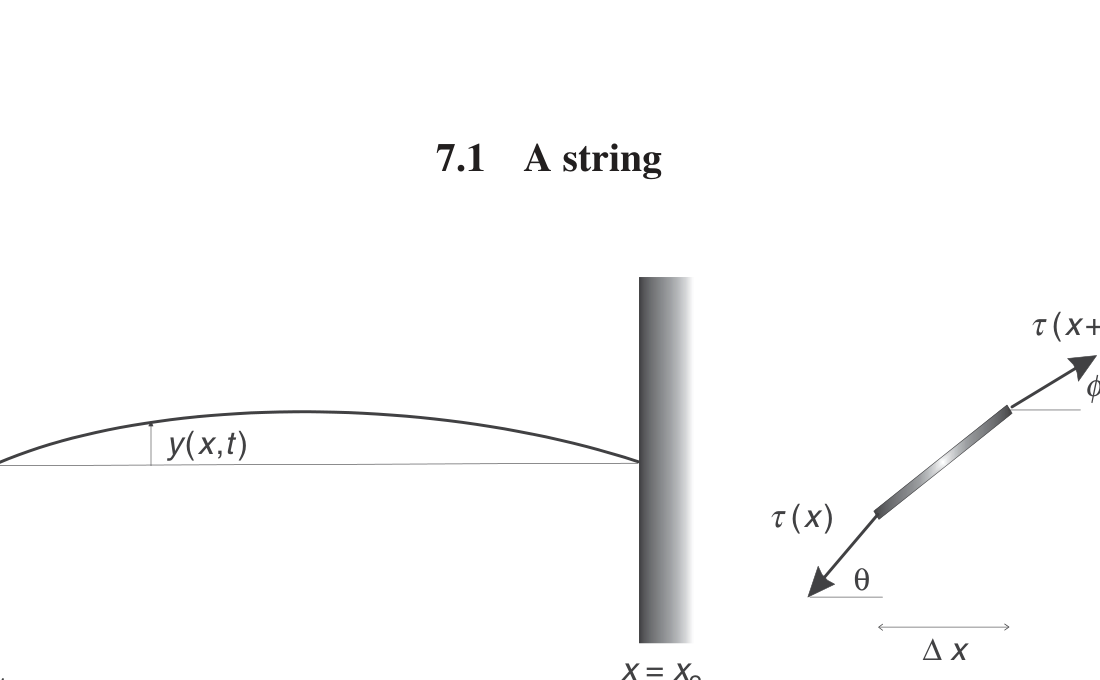
\includegraphics[width=0.55\linewidth]{../Figures/fig_7_1.png}
\caption{Figure 7.1}
\end{figure}

At instant t the displacement of the string at location x is y = y(x, t). Before
treating this problem from a variational point of view, let us briefly go through
the elementary derivation of the wave equation using Newton's second law.
Consider an element of the string of length dx. Its mass is \textbackslash{}lambda dx. The forces
acting on it are the tension on either end, that is, \textbackslash{}tau (x) and \textbackslash{}tau (x + dx), as
\begin{figure}[h]
\centering
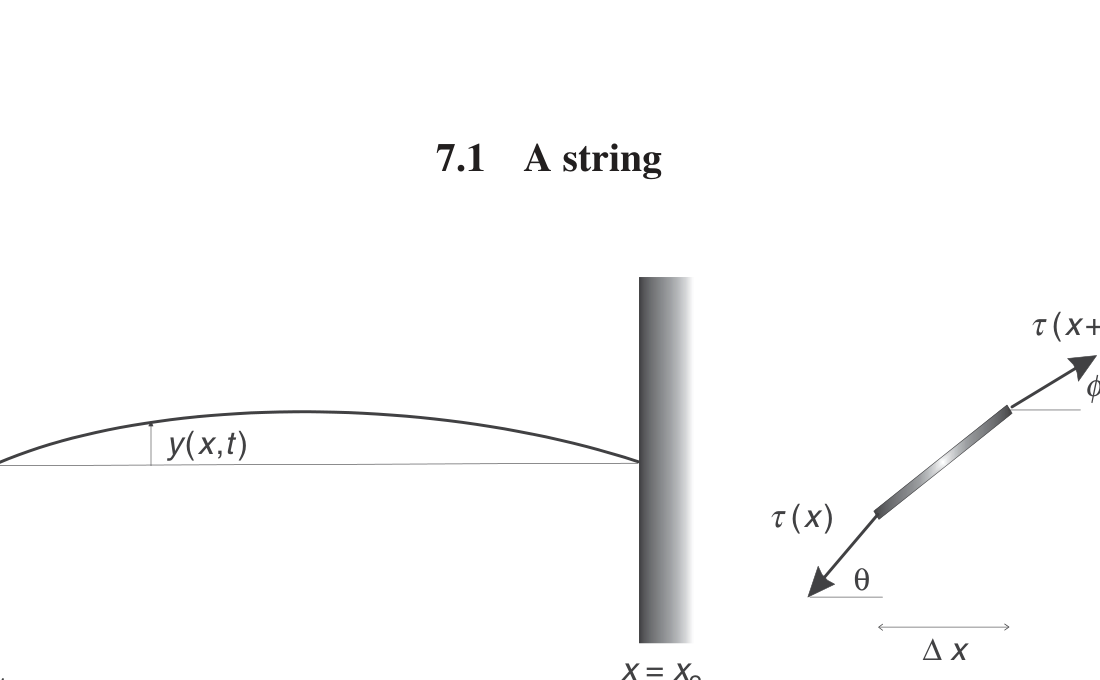
\includegraphics[width=0.55\linewidth]{../Figures/fig_7_1.png}
\caption{Figure 7.1}
\end{figure}

The figures are highly exaggerated, the string lies very close to the horizontal
x axis. Therefore,
sin \textbackslash{}theta  ≃tan \textbackslash{}theta  = lim
x\textbackslash{}to 0
y
x = \textbackslash{}partial y(x, t)
\textbackslash{}partial x
.
From ma = F we have
\textbackslash{}lambda (x)dx \textbackslash{}partial 2y
\textbackslash{}partial t2 = \textbackslash{}tau (x + dx) sin \textbackslash{}phi  -\textbackslash{}tau (x) sin \textbackslash{}theta
= \textbackslash{}tau (x + dx)\textbackslash{}partial y(x + dx, t)
\textbackslash{}partial x
-\textbackslash{}tau (x)\textbackslash{}partial y(x, t)
\textbackslash{}partial x
= \textbackslash{}tau (x)\textbackslash{}partial y(x, t)
\textbackslash{}partial x
+ dx

\textbackslash{}tau (x)\textbackslash{}partial y(x, t)
\textbackslash{}partial x

+ \textbackslash{}cdot  \textbackslash{}cdot  \textbackslash{}cdot  -\textbackslash{}tau (x)\textbackslash{}partial y(x, t)
\textbackslash{}partial x
\textbackslash{}lambda (x)dx \textbackslash{}partial 2y
\textbackslash{}partial t2 = \textbackslash{}partial
\textbackslash{}partial x

\textbackslash{}tau (x)\textbackslash{}partial y
\textbackslash{}partial x

,
(7.1)
where we expanded the first term in a Taylor's series.

For simplicity, let us assume that \textbackslash{}lambda  and T are not functions of x. Then
\textbackslash{}partial 2y
\textbackslash{}partial t2 = \textbackslash{}tau
\textbackslash{}lambda
\textbackslash{}partial 2y
\textbackslash{}partial x2 ,
which is the wave equation. The speed of the wave is \textbackslash{}sqrt\textbackslash{}lambda /T \textbackslash{}tau .
Thus we see that F = ma leads us to the wave equation. But we are interested in obtaining this result using Lagrangian methods. I will write the appropriate Lagrangian for the continuous string by introducing a Lagrangian per
unit length, or a Lagrangian density, which will be denoted L. The Lagrangian
for the system is
L =
x2
x1
Ldx.
It is easy to appreciate that the kinetic energy density of an element of the
string can be expressed as 1
2\textbackslash{}lambda dx $\textbackslash{}dot y$2, where \textbackslash{}lambda dx is the mass of the element of
length dx, and $\textbackslash{}dot y$ is its vertical velocity. It is not as obvious what to use for the
potential energy. But note that the force \textbackslash{}partial
\textbackslash{}partial x

\textbackslash{}tau (x) \textbackslash{}partial y
\textbackslash{}partial x

is related to the potential
energy through F = -\textbackslash{}partial V
\textbackslash{}partial x , so the potential energy can be written as 1
2\textbackslash{}tau y′2dx,
where y′ = \textbackslash{}partial y/\textbackslash{}partial x. Then the Lagrangian for the system can be written as
L =
x2
x1
Ldx =
x2
x1
2\textbackslash{}lambda (x) $\textbackslash{}dot y$2 -1
2\textbackslash{}tau (x)y′2

dx.
If we make the reasonable assumption that the mass density \textbackslash{}lambda  and the tension
\textbackslash{}tau  are constants, we obtain
L = \textbackslash{}lambda
x2
x1
$\textbackslash{}dot y$2dx -\textbackslash{}tau
x2
x1
y′2dx
and so, the Lagrangian density for this system is
L =\textbackslash{}lambda
2 $\textbackslash{}dot y$2 -\textbackslash{}tau
2y′2.
This is often written in a more explicit form as
L =\textbackslash{}lambda
\textbackslash{}partial y
\textbackslash{}partial t
-\textbackslash{}tau
\textbackslash{}partial y
\textbackslash{}partial x
.
(7.2)
\begin{exercise}
Exercise 7.1 Show that if the potential energy is given by 1
2\textbackslash{}tau y′2, the force
is given by the expression on the right-hand side of Equation (7.1).
\end{exercise}

\begin{exercise}
Exercise 7.2 Consider a traveling wave in a string described in the usual
way by y(x, t) = A cos(kx -\textbackslash{}omega t). How are k and \textbackslash{}omega  related to \textbackslash{}lambda  and \textbackslash{}tau ?

7.1
A string
Next let us determine the appropriate form for Lagrange's equations for this
system. Going back to fundamentals, we recall that Lagrange's equation is a
consequence of Hamilton's principle which we have stated as
\textbackslash{}delta
t2
t1
Ldt = 0.
That is, the variation of the action taken between end points t1 and t2 is zero.
But for our distributed one-dimensional system the Lagrangian may vary with
position along the string. (It is obvious that the velocity of a mass point in the
string depends on both t and x.) Assuming that the Lagrangian is distributed,
the total Lagrangian of the system is
L =
x2
x1
Ldx,
and Hamilton's principle then becomes
\textbackslash{}delta
t2
t1

x2
x1

dt = 0.
Let us consider the functional dependence of the Lagrangian density. It will be
depend explicitly on position and time (x and t), as these are the independent
variables. But we expect that it will depend implicitly on y, the displacement,
$\textbackslash{}dot y$ =
\textbackslash{}partial y
\textbackslash{}partial t , the velocity in the vertical direction, and y′ =
\textbackslash{}partial y
\textbackslash{}partial x , the ``stretch.''
That is,
L = L(y, $\textbackslash{}dot y$, y′; x, t).
Note that the independent variables x and t are the variables of integration in
Hamilton's principle. The Lagrangian density at a particular place and time
will, in general, depend on y, $\textbackslash{}dot y$, and y′. We can consider y to be a generalized
coordinate that specifies the configuration of the system. It will be varied in
Hamilton's principle. Its variation at the end points must be zero. But now we
have two sets of end points, both position and time. Note that we are not stating
that y itself is zero at the boundaries, only that its variation at the boundaries
is zero. That is,
\textbackslash{}delta (y(t1)) = \textbackslash{}delta (y(t2)) = 0,
and
\textbackslash{}delta (y(x1)) = \textbackslash{}delta (y(x2)) = 0.
This simply means that we require that all ``paths'' y(x, t) begin at (x1, t1)
and end at (x2, t2). For example, at the initial time, all locations on the varied

string configuration correspond to the actual initial configuration, and at all
times the varied string configuration has end points corresponding to the actual
configuration (which happen to be y(x1, t) = 0 and y(x2, t) = 0).
Hamilton's principle is
0 = \textbackslash{}delta
t2
t1
Ldt = \textbackslash{}delta
t2
t1
dt
x2
x1
dxL(y, y′, $\textbackslash{}dot y$; x, t)
0 =
t2
t1
dt
x2
x1

\textbackslash{}partial L
\textbackslash{}partial y \textbackslash{}delta y + \textbackslash{}partial L
\textbackslash{}partial y′ \textbackslash{}delta y′ + \textbackslash{}partial L
\textbackslash{}partial $\textbackslash{}dot y$ \textbackslash{}delta  $\textbackslash{}dot y$

.
(7.3)
Note that
\textbackslash{}delta y′ = \textbackslash{}delta  \textbackslash{}partial y
\textbackslash{}partial x = \textbackslash{}partial
\textbackslash{}partial x \textbackslash{}delta y,
where t is held fixed,
and
\textbackslash{}delta  $\textbackslash{}dot y$ = \textbackslash{}delta  \textbackslash{}partial y
\textbackslash{}partial t = \textbackslash{}partial
\textbackslash{}partial t \textbackslash{}delta y,
where x is held fixed.
Consider the first term in Equation (7.3), keeping in mind that y (and $\textbackslash{}dot y$) are
values along the varied path (expressed, for example, as Y in Equation (2.5)):
t2
t1
dt
x2
x1

\textbackslash{}partial L
\textbackslash{}partial $\textbackslash{}dot y$ \textbackslash{}delta  $\textbackslash{}dot y$

=
t2
t1
dt
x2
x1

\textbackslash{}partial L
\textbackslash{}partial $\textbackslash{}dot y$
\textbackslash{}partial $\textbackslash{}dot y$
\textbackslash{}partial ϵ \textbackslash{}delta ϵ

=
x2
x1
t2
t1
dt

\textbackslash{}partial L
\textbackslash{}partial $\textbackslash{}dot y$
\textbackslash{}partial $\textbackslash{}dot y$
\textbackslash{}partial ϵ \textbackslash{}delta ϵ

=
x2
x1
t2
t1
dt \textbackslash{}partial L
\textbackslash{}partial $\textbackslash{}dot y$
\textbackslash{}partial
\textbackslash{}partial ϵ
\textbackslash{}partial y
\textbackslash{}partial t

\textbackslash{}delta ϵ
=
x2
x1
t2
t1
\textbackslash{}partial L
\textbackslash{}partial $\textbackslash{}dot y$
\textbackslash{}partial
\textbackslash{}partial t
\textbackslash{}partial y
\textbackslash{}partial ϵ dt\textbackslash{}delta ϵ.
Integrating by parts
t2
t1
dt
x2
x1

\textbackslash{}partial L
\textbackslash{}partial $\textbackslash{}dot y$ \textbackslash{}delta  $\textbackslash{}dot y$

=
x2
x1
dx\textbackslash{}delta ϵ
!
\textbackslash{}partial L
\textbackslash{}partial $\textbackslash{}dot y$
\textbackslash{}partial y
\textbackslash{}partial ϵ
t2
t1
-
t2
t1
\textbackslash{}partial
\textbackslash{}partial t
\textbackslash{}partial L
\textbackslash{}partial $\textbackslash{}dot y$
\textbackslash{}partial y
\textbackslash{}partial ϵ dt
"
=
x2
x1
\#
0 -
t2
t1
\textbackslash{}partial
\textbackslash{}partial t
\textbackslash{}partial L
\textbackslash{}partial $\textbackslash{}dot y$
\textbackslash{}partial y
\textbackslash{}partial ϵ \textbackslash{}delta ϵdt
$
=
x2
x1
\#
-
t2
t1
\textbackslash{}partial
\textbackslash{}partial t
\textbackslash{}partial L
\textbackslash{}partial $\textbackslash{}dot y$ \textbackslash{}delta ydt
$
= -
t2
t1
dt
x2
x1
\textbackslash{}partial
\textbackslash{}partial t
\textbackslash{}partial L
\textbackslash{}partial $\textbackslash{}dot y$

\textbackslash{}delta y.

7.1
A string
Similarly, we can integrate the second term in Equation (7.3) by parts to obtain
t2
t1
dt
x2
x1

\textbackslash{}partial L
\textbackslash{}partial y′ \textbackslash{}delta y′

=
t2
t1
x2
x1
dtdx(-1) \textbackslash{}partial
\textbackslash{}partial x
\textbackslash{}partial L
\textbackslash{}partial y′ ,
where we used the fact that the variation vanishes at the end points.
In conclusion, we appreciate that Hamilton's principle can be expressed as
0 =
t2
t1
dt
x2
x1

\textbackslash{}partial L
\textbackslash{}partial y -\textbackslash{}partial
\textbackslash{}partial x
\textbackslash{}partial L
\textbackslash{}partial y′ -\textbackslash{}partial
\textbackslash{}partial t
\textbackslash{}partial L
\textbackslash{}partial $\textbackslash{}dot y$

\textbackslash{}delta y.
As usual, Hamilton's principle leads to the Lagrange equations. In the preceding equation we note that the variation \textbackslash{}delta y is arbitrary so the term in brackets
must be zero. Thus we obtain the general form for Lagrange's equations for a
one-dimensional continuous system:
\textbackslash{}partial
\textbackslash{}partial x
\textbackslash{}partial L
\textbackslash{}partial $\textbackslash{}dot y$ + \textbackslash{}partial
\textbackslash{}partial t
\textbackslash{}partial L
\textbackslash{}partial y′ -\textbackslash{}partial L
\textbackslash{}partial y = 0.
(7.4)
We can write this in a more explicit but more complicated form as
\textbackslash{}partial
\textbackslash{}partial x
\textbackslash{}partial L
\textbackslash{}partial

\textbackslash{}partial y
\textbackslash{}partial t
+ \textbackslash{}partial
\textbackslash{}partial t
\textbackslash{}partial L
\textbackslash{}partial

\textbackslash{}partial y
\textbackslash{}partial x
-\textbackslash{}partial L
\textbackslash{}partial y = 0.
As a simple application, let us apply this form of the Lagrange equation to
the Lagrangian density for a string which is
L =\textbackslash{}lambda
\textbackslash{}partial y
\textbackslash{}partial t
-\textbackslash{}tau
\textbackslash{}partial y
\textbackslash{}partial x
.
We appreciate that
\textbackslash{}partial L
\textbackslash{}partial $\textbackslash{}dot y$ = \textbackslash{}lambda  $\textbackslash{}dot y$,
\textbackslash{}partial L
\textbackslash{}partial y′ = -\textbackslash{}tau y′,
and
\textbackslash{}partial L
\textbackslash{}partial y = 0,
so that Equation (7.4) yields
\textbackslash{}partial
\textbackslash{}partial t (\textbackslash{}lambda  $\textbackslash{}dot y$) + \textbackslash{}partial
\textbackslash{}partial x

-\textbackslash{}tau y′
= 0,
\textbackslash{}lambda $\textbackslash{}ddot y$ -\textbackslash{}tau y′′ = 0.
That is,
\textbackslash{}partial 2y
\textbackslash{}partial t2 = \textbackslash{}tau
\textbackslash{}lambda
\textbackslash{}partial 2y
\textbackslash{}partial x2 ,
the wave equation.

\end{exercise}

\section*{7.2  Generalization to three dimensions}

We expressed the Lagrangian density for a one-dimensional system as
L = L(y, $\textbackslash{}dot y$, y′; x, t),
or
L = L

y, \textbackslash{}partial y
\textbackslash{}partial t , \textbackslash{}partial y
\textbackslash{}partial x ; x, t

.
Generalizing to three dimensions, let the configuration of the system be
specified by a scalar coordinate w = w(x, y, z, t). We shall replace y with
w and $\textbackslash{}dot y$ with $\textbackslash{}dot w$ = \textbackslash{}partial w
\textbackslash{}partial t . This is straightforward. But now we need to replace y′
with the derivatives of w with respect to x, y, z, specifically with \textbackslash{}partial w
\textbackslash{}partial x , \textbackslash{}partial w
\textbackslash{}partial y , \textbackslash{}partial w
\textbackslash{}partial z .
Recalling the vector identity, \textbackslash{}nabla w = ˆx \textbackslash{}partial w
\textbackslash{}partial x +ˆy \textbackslash{}partial w
\textbackslash{}partial y +ˆz \textbackslash{}partial w
\textbackslash{}partial z we see that a reasonably
compact notation could be to let \textbackslash{}partial w
\textbackslash{}partial x be represented as the x component of \textbackslash{}nabla w,
thus,
\textbackslash{}partial w
\textbackslash{}partial x = \textbackslash{}nabla xw,
and similarly for the other two components. Then we write
L = L

w, \textbackslash{}partial w
\textbackslash{}partial t , \textbackslash{}nabla w; x, y, z, t

,
or
L = L

w, \textbackslash{}partial w
\textbackslash{}partial t , \textbackslash{}nabla xw, \textbackslash{}nabla yw, \textbackslash{}nabla zw; x,t

,
where x is the vector with components x, y, z = x1, x2, x3.
The condition that the end points are fixed in time is
\textbackslash{}delta w(t1) = \textbackslash{}delta w(t2) = 0.
The Lagrange equation is, then,
\textbackslash{}partial
\textbackslash{}partial t

\textbackslash{}partial L
\textbackslash{}partial
\textbackslash{}partial w
\textbackslash{}partial t


+
i=1
\textbackslash{}partial
\textbackslash{}partial $\textbackslash{}xi$
⎛
⎝
\textbackslash{}partial L
\textbackslash{}partial

\textbackslash{}partial w
\textbackslash{}partial $\textbackslash{}xi$

⎞
⎠-\textbackslash{}partial L
\textbackslash{}partial w = 0,
(7.5)
or, more compactly
\textbackslash{}partial
\textbackslash{}partial t
\textbackslash{}partial L
\textbackslash{}partial $\textbackslash{}dot w$

+ \textbackslash{}partial
\textbackslash{}partial $\textbackslash{}xi$

\textbackslash{}partial L
\textbackslash{}partial (\textbackslash{}nabla iw)

-\textbackslash{}partial L
\textbackslash{}partial w = 0,
(7.6)
where the summation in the middle term has been replaced by the summation
convention.

7.3
The Hamiltonian density
\section*{7.3  The Hamiltonian density}

Returning to a one-dimensional system, we consider the Hamiltonian density
H, which bears the same relationship to the Lagrangian density L that the
Hamiltonian H bears to the Lagrangian L, namely H = p $\textbackslash{}dot q$ -L.
For a one-dimensional continuous system we can write $\textbackslash{}dot Q\_ instead of $\textbackslash{}dot q$,
recalling that $\textbackslash{}dot q$ = $\textbackslash{}dot q$(t) is the generalized velocity of a particle, whereas
$\textbackslash{}dot Q\_ =
$\textbackslash{}dot Q\_(x, t) is a distributed quantity that depends on the entire range of
positions.
To carry out our analogy between Hamiltonian density and Hamiltonian we
need to define a distributed or continous variable analogous to the momentum.
Based on the usual definition of generalized momentum as p = \textbackslash{}partial L/\textbackslash{}partial $\textbackslash{}dot q$ we
define the canonical momentum density by
P = \textbackslash{}partial L
\textbackslash{}partial $\textbackslash{}dot Q\_.
Then the one-dimensional Hamiltonian density is
H = P $\textbackslash{}dot Q\_-L.
Let us now generalize to a three-dimensional system described by the configuration parameter Q. For convenience, let the Lagrange density not depend
explicitly on t, (but it depends implicitly on time through the time dependence
of Q). So,
L = L(Q, $\textbackslash{}dot Q\_, Q′
x, Q′
y, Q′
z; x).
We are using a time-independent Lagrangian density because we want to
explore the conservation of energy which involves investigating the partial
derivative of H with respect to time:
\textbackslash{}partial H
\textbackslash{}partial t = \textbackslash{}partial
\textbackslash{}partial t

P $\textbackslash{}dot Q\_-L

\textbackslash{}partial H
\textbackslash{}partial t = \textbackslash{}partial P
\textbackslash{}partial t
\textbackslash{}partial Q
\textbackslash{}partial t + P \textbackslash{}partial 2Q
\textbackslash{}partial t2 -

\textbackslash{}partial L
\textbackslash{}partial Q
\textbackslash{}partial Q
\textbackslash{}partial t + \textbackslash{}partial L
\textbackslash{}partial $\textbackslash{}dot Q\_
\textbackslash{}partial $\textbackslash{}dot Q\_
\textbackslash{}partial t +
k=1
\textbackslash{}partial L
\textbackslash{}partial Q′
k
\textbackslash{}partial Q′
k
\textbackslash{}partial t

. (7.7)
But
\textbackslash{}partial P
\textbackslash{}partial t = \textbackslash{}partial
\textbackslash{}partial t
\textbackslash{}partial L
\textbackslash{}partial $\textbackslash{}dot Q\_,
and Lagrange's equation tells us that
\textbackslash{}partial
\textbackslash{}partial t
\textbackslash{}partial L
\textbackslash{}partial $\textbackslash{}dot Q\_ = \textbackslash{}partial L
\textbackslash{}partial Q -
k=1
\textbackslash{}partial
\textbackslash{}partial xk
\textbackslash{}partial L
\textbackslash{}partial Q′
k
,

so
\textbackslash{}partial P
\textbackslash{}partial t = \textbackslash{}partial L
\textbackslash{}partial Q -
k=1
\textbackslash{}partial
\textbackslash{}partial xk
\textbackslash{}partial L
\textbackslash{}partial Q′
k
.
Plugging into Equation (7.7) we get
\textbackslash{}partial H
\textbackslash{}partial t =

\textbackslash{}partial L
\textbackslash{}partial Q -
k=1
\textbackslash{}partial
\textbackslash{}partial xk
\textbackslash{}partial L
\textbackslash{}partial Q′
k

\textbackslash{}partial Q
\textbackslash{}partial t + P \textbackslash{}partial 2Q
\textbackslash{}partial t2 -

\textbackslash{}partial L
\textbackslash{}partial Q
\textbackslash{}partial Q
\textbackslash{}partial t + \textbackslash{}partial L
\textbackslash{}partial $\textbackslash{}dot Q\_
\textbackslash{}partial $\textbackslash{}dot Q\_
\textbackslash{}partial t
+
k=1
\textbackslash{}partial L
\textbackslash{}partial Q′
k
\textbackslash{}partial
\textbackslash{}partial t
\textbackslash{}partial Q
\textbackslash{}partial xk

.
The first and fourth terms on the left cancel. Furthermore, the second term on
the left can be expressed as:

k=1
\textbackslash{}partial
\textbackslash{}partial xk
\textbackslash{}partial L
\textbackslash{}partial Q′
k

\textbackslash{}partial Q
\textbackslash{}partial t =
k=1
\textbackslash{}partial
\textbackslash{}partial xk
\textbackslash{}partial L
\textbackslash{}partial Q′
k
\textbackslash{}partial Q
\textbackslash{}partial t

-
k=1
\textbackslash{}partial L
\textbackslash{}partial Q′
k
\textbackslash{}partial
\textbackslash{}partial xk
\textbackslash{}partial Q
\textbackslash{}partial t ,
leaving us with
\textbackslash{}partial H
\textbackslash{}partial t = P \textbackslash{}partial 2Q
\textbackslash{}partial t2 -
k=1
\textbackslash{}partial
\textbackslash{}partial xk
\textbackslash{}partial L
\textbackslash{}partial Q′
k
\textbackslash{}partial Q
\textbackslash{}partial t

+ \textbackslash{}partial L
\textbackslash{}partial $\textbackslash{}dot Q\_
\textbackslash{}partial $\textbackslash{}dot Q\_
\textbackslash{}partial t ,
\textbackslash{}partial H
\textbackslash{}partial t = -
k=1
\textbackslash{}partial
\textbackslash{}partial xk
\textbackslash{}partial L
\textbackslash{}partial Q′
k
\textbackslash{}partial Q
\textbackslash{}partial t

.
It is interesting to write the right-hand side as -\textbackslash{}nabla\textbackslash{}cdot -\textbackslash{}to
S, where Si
=
\textbackslash{}partial
\textbackslash{}partial xk

\textbackslash{}partial L
\textbackslash{}partial Q′
k
\textbackslash{}partial Q
\textbackslash{}partial t

. Then
\textbackslash{}partial H
\textbackslash{}partial t + \textbackslash{}nabla\textbackslash{}cdot  -\textbackslash{}to
S = 0,
which we recognize as an equation of continuity, expressing the conservation
of energy. This can be appreciated better by integrating over the volume of our
system. Since H =

\textbackslash{}int H\textbackslash{},d\^3x we can write
dH
dt =

\textbackslash{}partial H
\textbackslash{}partial t d\^3x = -

\textbackslash{}nabla\textbackslash{}cdot -\textbackslash{}to
S d\^3x
and applying the divergence theorem we obtain
dH
dt = -

A
-\textbackslash{}to
S \textbackslash{}cdot  ˆnda,
(7.8)
where A is the area of the surface. This tells us that a change in the energy
contained in a volume is accompanied by a flow of energy across the surface

7.3
The Hamiltonian density
bounding the volume. Thus -\textbackslash{}to
S is an energy flux density.1 If the surface is at
infinity, the right hand side of Equation (7.8) is zero and the Hamiltonian is
constant. An example might be an infinite system which is perturbed at some
location. The Hamiltonian is also constant if -\textbackslash{}to
S is perpendicular to the bounding surface so that -\textbackslash{}to
S \textbackslash{}cdot  ˆn = 0. An example would be a finite string with fixed
end points.
\begin{exercise}
Exercise 7.3 For a one-dimensional string, L is given by Equation (7.2).
Show that -\textbackslash{}to
S is given by -\textbackslash{}to
S = -\textbackslash{}tau  \textbackslash{}partial y
\textbackslash{}partial x
\textbackslash{}partial y
\textbackslash{}partial t ˆx. Explain the direction of -\textbackslash{}to
S.
Show that the energy flux is zero at the end points (x1 and x2).
Revisiting the string
If we apply the concepts of discrete mechanics to the string, we would write
the relation between the Lagrange density, the kinetic energy density and the
potential energy density in the form:
L = T -V.
As we have seen, the kinetic energy density is
T = 1
2\textbackslash{}lambda
\textbackslash{}partial y
\textbackslash{}partial t
= 1
2\textbackslash{}lambda  $\textbackslash{}dot y$2.
Since the potential energy does not depend on the velocity we have
\textbackslash{}partial V
\textbackslash{}partial $\textbackslash{}dot y$ = 0
and consequently the generalized momentum density is
P = \textbackslash{}partial L
\textbackslash{}partial $\textbackslash{}dot y$ = \textbackslash{}lambda \textbackslash{}partial y
\textbackslash{}partial t .
Then
H = P $\textbackslash{}dot y$-L = 2T -(T -V) = T + V
as expected.
The Lagrangian density of the oscillating string is
L = \textbackslash{}lambda (x)
\textbackslash{}partial y
\textbackslash{}partial t
-\textbackslash{}tau (x)
\textbackslash{}partial y
\textbackslash{}partial x
= \textbackslash{}lambda (x)
$\textbackslash{}dot y$2 -\textbackslash{}tau (x)
2 y′2.
1 Note the relationship to electromagnetism and the Poynting vector.

Denoting y by Q we can write
L = 1
2\textbackslash{}lambda  $\textbackslash{}dot Q\_2-1
2\textbackslash{}tau Q′2
P = \textbackslash{}partial L
\textbackslash{}partial $\textbackslash{}dot Q\_ = \textbackslash{}lambda (x) $\textbackslash{}dot Q\_.
Consequently,
H = P $\textbackslash{}dot Q\_-L,
and
-\textbackslash{}to
S = \textbackslash{}partial L
\textbackslash{}partial Q′ $\textbackslash{}dot Q\_ = -\textbackslash{}tau (x)Q′ $\textbackslash{}dot Q\_ˆx.
This is the energy flux vector, that is, the rate at which energy flows along the
string.
\end{exercise}

\begin{exercise}
Exercise 7.4 If y = A cos(kx -\textbackslash{}omega t) (which is a traveling wave moving
towards the right), show that
Sx = A2(\textbackslash{}tau kc) sin2(kx -\textbackslash{}omega t)
and that
⟨Sx⟩= 1
2A2\textbackslash{}lambda c\textbackslash{}omega 2,
where c2 = \textbackslash{}lambda /\textbackslash{}tau  and k = \textbackslash{}omega /c.
\end{exercise}

\section*{7.4  Another one-dimensional system}

We now consider a different one-dimensional system. Although there are great
similarities beween the two one-dimensional systems, we shall use the second
system to elucidate some concepts that have not been brought out yet.
Imagine taking a hammer and hitting a large solid block of iron. A threedimensional pressure/density wave will propagate through the solid. The perturbed molecules will be acted upon by intermolecular forces tending to bring
them back to their equilibrium positions. We could, in principle, follow the
motions of the individual molecules, but clearly it is advantageous to treat the
iron block as a continuous system described by continuous parameters such as
the density as a function of position and time.

7.4
Another one-dimensional system
a
k
k
k
k
a
a
$\textbackslash{}xi$+1
Beads of mass m on a thin, stiff wire, connected by springs of constant k. The equilibrium separation distance is a. The lower figure shows two
beads displaced from equilibrium by distances \textbackslash{}xi i and \textbackslash{}xi i+1.
To better understand the physics of such a system it is convenient to begin
with a one-dimensional system consisting of particles aligned in a straight line.
Our ``toy model'' can be imagined as beads mounted on a thin rigid wire and
\begin{figure}[h]
\centering
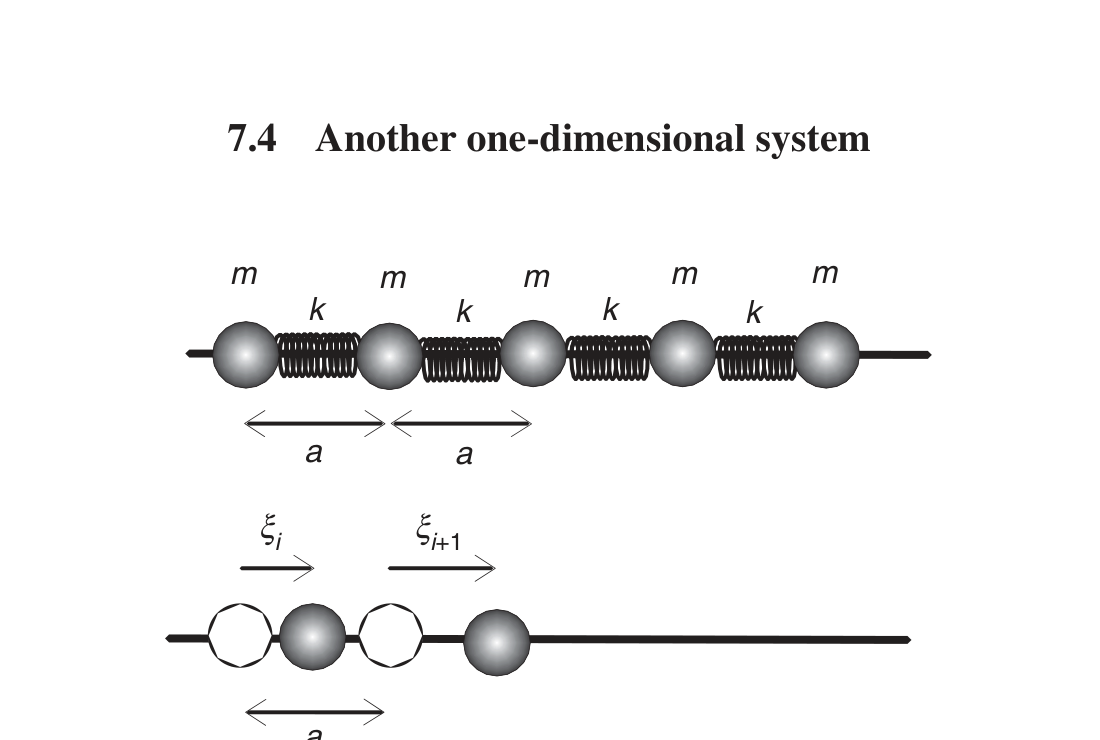
\includegraphics[width=0.55\linewidth]{../Figures/fig_7_2.png}
\caption{Figure 7.2}
\end{figure}

Let each bead have mass m and each spring have spring constant k. Let the
equilibrium spacing of the beads be a. If the equilibrium position of the ith
bead is $\textbackslash{}xi$, then its position when disturbed from equilibrium can be denoted
\begin{figure}[h]
\centering
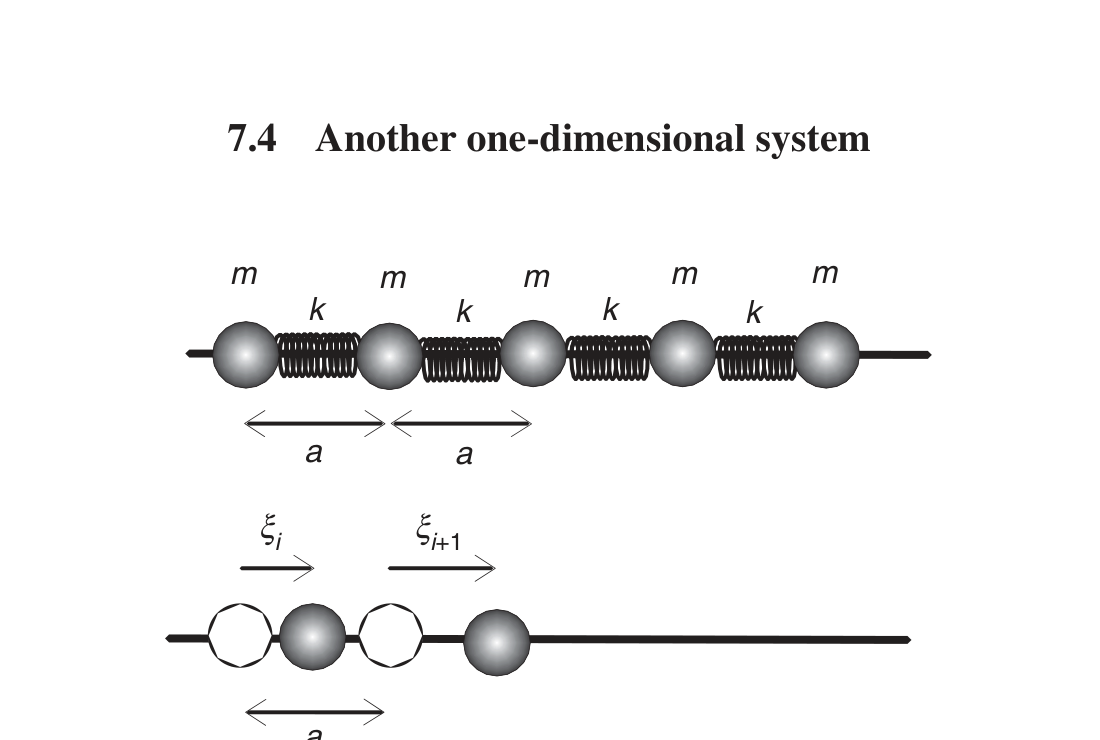
\includegraphics[width=0.55\linewidth]{../Figures/fig_7_2.png}
\caption{Figure 7.2}
\end{figure}

and particle i +1 is a +\textbackslash{}xi i+1 -\textbackslash{}xi i. The natural length of the springs is a, so the
stretch of the spring is (\textbackslash{}xi i+1 -\textbackslash{}xi i) and the potential energy associated with the
spring is 1
2k(\textbackslash{}xi i+1 -\textbackslash{}xi i)2. The velocity of particle i relative to its equilibrium
position (which is assumed to be at rest) is simply $\textbackslash{}dot\textbackslash{}$xi i. Using these concepts we
can write the Lagrangian in the usual form as
L = T -V =
2mi $\textbackslash{}dot\textbackslash{}$xi 2
i -1
2k(\textbackslash{}xi i+1 -\textbackslash{}xi i)2

.
(7.9)
\begin{exercise}
Exercise 7.5 Using the Lagrangian given in Equation (7.9), show that the
equations of motion for this system of discrete particles are
mi $\textbackslash{}ddot \textbackslash{}xi$ i -k(\textbackslash{}xi i+1 -\textbackslash{}xi i) + k(\textbackslash{}xi i -\textbackslash{}xi i-1) = 0.

7.4.1 The limit of a continuous rod
We now represent the system of beads as a continuous system. We begin by
multiplying and dividing Equation (7.9) by a, thus:
L = a

a
$\textbackslash{}dot\textbackslash{}$xi 2
i -1
2ka
\textbackslash{}xi i+1 -\textbackslash{}xi i
a
.
As a \textbackslash{}to 0, mi/a \textbackslash{}to \textbackslash{}lambda (x), the mass per unit length, i.e. the linear mass density
of the rod at location x. The term \textbackslash{}xi i+1-\textbackslash{}xi i
a
can be written as a continuous function also. Let \textbackslash{}xi i = \textbackslash{}xi (x) and \textbackslash{}xi i+1 = \textbackslash{}xi (x + a). For convenience, let us write
x for a. Then
\textbackslash{}xi i+1 -\textbackslash{}xi i
a
\textbackslash{}to \textbackslash{}xi (x + x) -\textbackslash{}xi (x)
and, in the limit a \textbackslash{}to 0,
\textbackslash{}xi i+1 -\textbackslash{}xi i
a
\textbackslash{}to d\textbackslash{}xi
and
ka
\textbackslash{}xi i+1 -\textbackslash{}xi i
a
\textbackslash{}to kx
\textbackslash{}partial \textbackslash{}xi
\textbackslash{}partial x
.
The summation becomes an integral over x, and
L = 1

\textbackslash{}lambda (x)
\textbackslash{}partial \textbackslash{}xi
\textbackslash{}partial t
-K
\textbackslash{}partial \textbackslash{}xi
\textbackslash{}partial x
dx.
(7.10)
\end{exercise}

\begin{exercise}
Exercise 7.6 Show that K is Young's modulus.
\end{exercise}

\begin{exercise}
Exercise 7.7 Show that the Lagrangian in Equation (7.10) yields the wave
equation.
Let us apply Hamilton's principle and derive Lagrange's equation. (This
derivation is similar to our previous considerations with the string.)
According to Hamilton's principle,
\textbackslash{}delta
t2
t1

x2
x1

dt = 0,
where L = L(\textbackslash{}xi , $\textbackslash{}dot\textbackslash{}$xi , \textbackslash{}xi ′). For the problem at hand, the quantity being varied is \textbackslash{}xi
and not x or t. Therefore, the variation of \textbackslash{}xi  at the end points is zero where the
end points are not only t1 and t2 but also x1 and x2.

7.4
Another one-dimensional system
When we express \textbackslash{}xi  as a continuous variable it is interpreted as representing
the displacement from equilibrium of an infinitesimal segment of the rod. (This
is difficult to visualize, so perhaps it is helpful to have a mental image of \textbackslash{}xi  as
representing some other variable such as the density.)
To apply the variational method, we need to imagine a varied quantity
\textbackslash{}xi (x, t, ϵ) which differs infinitesimally from the ``true'' quantity \textbackslash{}xi (x, t, 0). That
is, we define
\textbackslash{}xi (x, t, ϵ) = \textbackslash{}xi (x, t, 0) + ϵ\textbackslash{}eta (x, t),
where \textbackslash{}xi (x, t, 0) is the ``true'' path, ϵ is a small parameter, and \textbackslash{}eta (x, t) is an
arbitrary function that is zero at the end points. That is,
\textbackslash{}eta (x1, t1) = 0,
and
\textbackslash{}eta (x2, t2) = 0.
Following the usual prescription, we write
dϵ =
t2
t1
dt
x2
x1

\textbackslash{}partial L
\textbackslash{}partial \textbackslash{}xi
\textbackslash{}partial \textbackslash{}xi
\textbackslash{}partial ϵ + \textbackslash{}partial L
\textbackslash{}partial $\textbackslash{}dot\textbackslash{}$xi
\textbackslash{}partial $\textbackslash{}dot\textbackslash{}$xi
\textbackslash{}partial ϵ + \textbackslash{}partial L
\textbackslash{}partial \textbackslash{}xi ′
\textbackslash{}partial \textbackslash{}xi ′
\textbackslash{}partial ϵ

= 0.
Integrating the second and third terms by parts we obtain
t2
t1
\textbackslash{}partial L
\textbackslash{}partial $\textbackslash{}dot\textbackslash{}$xi
\textbackslash{}partial $\textbackslash{}dot\textbackslash{}$xi
\textbackslash{}partial ϵ dt = -
t2
t1
\textbackslash{}partial
\textbackslash{}partial t
\textbackslash{}partial L
\textbackslash{}partial $\textbackslash{}dot\textbackslash{}$xi
\textbackslash{}partial \textbackslash{}xi
\textbackslash{}partial ϵ dt,
and
x2
x1
\textbackslash{}partial L
\textbackslash{}partial \textbackslash{}xi ′
\textbackslash{}partial \textbackslash{}xi ′
\textbackslash{}partial ϵ dx = -
x2
x1
\textbackslash{}partial
\textbackslash{}partial x
\textbackslash{}partial L
\textbackslash{}partial \textbackslash{}xi ′
\textbackslash{}partial \textbackslash{}xi
\textbackslash{}partial ϵ dx,
leading to
0 = dI
dϵ

ϵ=0
=
t2
t1
dt
x2
x1
\textbackslash{}partial L
\textbackslash{}partial \textbackslash{}xi  -\textbackslash{}partial
\textbackslash{}partial t
\textbackslash{}partial L
\textbackslash{}partial $\textbackslash{}dot\textbackslash{}$xi  -\textbackslash{}partial
\textbackslash{}partial x
\textbackslash{}partial L
\textbackslash{}partial \textbackslash{}xi ′
\textbackslash{}partial \textbackslash{}xi
\textbackslash{}partial ϵ

ϵ=0

.
Consequently, Lagrange's equations are
\textbackslash{}partial
\textbackslash{}partial t
\textbackslash{}partial L
\textbackslash{}partial $\textbackslash{}dot\textbackslash{}$xi

+ \textbackslash{}partial
\textbackslash{}partial x
\textbackslash{}partial L
\textbackslash{}partial \textbackslash{}xi ′

-\textbackslash{}partial L
\textbackslash{}partial \textbackslash{}xi  = 0,
(7.11)
as previously obtained (see Equation (7.4)).
It is interesting to note that for the discrete system we obtain one Lagrange
equation for each bead, whereas for the continuous system we obtain a single
Lagrange equation. On the other hand, we can consider that Equation (7.11) is
an infinite number of equations, one for each of the infinite number of possible
values of x.

\end{exercise}

\begin{exercise}
Exercise 7.8 Show that Equation (7.11) applied to Equation (7.10) leads
to the wave equation.
Generalization to three dimensions
As previously noted, we can easily generate the relations developed above to
three dimensions. This would entail replacing the scalar displacement \textbackslash{}xi  by a
vector displacement, \textbackslash{}xi , with components \textbackslash{}xi i, where i = (1, 2, 3) or (x, y, z).
The quantity \textbackslash{}xi  represents a physical quantity defined at every point in some
region of space, so it satisfies the definition of a field. In fact, we can let \textbackslash{}xi
represent some other physical quantity such as the pressure or velocity or electromagnetic field.
The field \textbackslash{}xi  is, consequently, defined at every point and at every instant of
time so \textbackslash{}xi  = \textbackslash{}xi (x, y, z, t) and the Lagrange equation is
\textbackslash{}partial
\textbackslash{}partial t
\textbackslash{}partial L
\textbackslash{}partial $\textbackslash{}dot\textbackslash{}$xi
+ \textbackslash{}partial
\textbackslash{}partial x

\textbackslash{}partial L
\textbackslash{}partial (\textbackslash{}partial \textbackslash{}xi /\textbackslash{}partial x)

+ \textbackslash{}partial
\textbackslash{}partial y

\textbackslash{}partial L
\textbackslash{}partial (\textbackslash{}partial \textbackslash{}xi /\textbackslash{}partial y)

+ \textbackslash{}partial
\textbackslash{}partial z

\textbackslash{}partial L
\textbackslash{}partial (\textbackslash{}partial \textbackslash{}xi /\textbackslash{}partial z)

-\textbackslash{}partial L
\textbackslash{}partial \textbackslash{}xi  = 0.
The ith component of this equation is
\textbackslash{}partial
\textbackslash{}partial t
\textbackslash{}partial L
\textbackslash{}partial (\textbackslash{}partial \textbackslash{}xi i/\textbackslash{}partial t) +
k=1
\textbackslash{}partial
\textbackslash{}partial xk
\textbackslash{}partial L
\textbackslash{}partial (\textbackslash{}partial \textbackslash{}xi i/\textbackslash{}partial xk) -\textbackslash{}partial L
\textbackslash{}partial \textbackslash{}xi i
= 0,
(7.12)
where xk = x, y, z. It might be noted that \textbackslash{}partial
\textbackslash{}partial t and
\textbackslash{}partial
\textbackslash{}partial xk are sometimes written as
the total derivatives d
dt and
dxk to indicate that during the differentiation one
must also include the implicit dependence of \textbackslash{}xi i on xk or t.
It may be helpful to use a simpler notation, such as $\textbackslash{}dot\textbackslash{}$xi i for \textbackslash{}partial \textbackslash{}xi i/\textbackslash{}partial t and \textbackslash{}xi ′
ik for
\textbackslash{}partial \textbackslash{}xi i/\textbackslash{}partial xk. Then Equation (7.12) is written as
\textbackslash{}partial
\textbackslash{}partial t
\textbackslash{}partial L
\textbackslash{}partial $\textbackslash{}dot\textbackslash{}$xi  +
k=1
\textbackslash{}partial
\textbackslash{}partial xk
\textbackslash{}partial L
\textbackslash{}partial (\textbackslash{}xi ′
ik) -\textbackslash{}partial L
\textbackslash{}partial \textbackslash{}xi i
= 0.
(7.13)
Simplified notation using the functional derivative
We can simplify the notation somewhat by using the functional derivative that
was defined by Equation (2.10) as
\textbackslash{}delta
\textbackslash{}delta y = \textbackslash{}partial
\textbackslash{}partial y -d
\textbackslash{}partial
\textbackslash{}partial y′ .

7.4
Another one-dimensional system
For our purposes we write this as
\textbackslash{}delta L
\textbackslash{}delta \textbackslash{}xi i
= \textbackslash{}partial L
\textbackslash{}partial \textbackslash{}xi i
-
k=1
dxk
\textbackslash{}partial L
\textbackslash{}partial \textbackslash{}nabla \textbackslash{}xi i
,
or
\textbackslash{}delta L
\textbackslash{}delta \textbackslash{}xi  = \textbackslash{}partial L
\textbackslash{}partial \textbackslash{}xi  -\textbackslash{}nabla\textbackslash{}cdot  \textbackslash{}partial L
\textbackslash{}partial \textbackslash{}nabla \textbackslash{}xi  .
Consequently, in terms of the functional derivative, Hamilton's principle,
0 = \textbackslash{}delta L =


\textbackslash{}partial L
\textbackslash{}partial \textbackslash{}xi i
\textbackslash{}delta \textbackslash{}xi i -
k=1
dxk
\textbackslash{}partial L
\textbackslash{}partial (\textbackslash{}partial \textbackslash{}xi i/\textbackslash{}partial xk) + \textbackslash{}partial L
\textbackslash{}partial $\textbackslash{}dot\textbackslash{}$xi i
\textbackslash{}delta $\textbackslash{}dot\textbackslash{}$xi i

d\^3x,
can be expressed as
\textbackslash{}delta L =

\textbackslash{}delta L
\textbackslash{}delta \textbackslash{}xi i
\textbackslash{}delta \textbackslash{}xi i + \textbackslash{}partial L
\textbackslash{}partial $\textbackslash{}dot\textbackslash{}$xi i
\textbackslash{}delta $\textbackslash{}dot\textbackslash{}$xi i

d\^3x.
For the sake of simplicity, and to make the preceding more intelligible,
let us go back to a one-dimensional system and a scalar variable, replacing
\textbackslash{}xi  by Q. Furthermore, let us define the generalized momentum density in the
usual way,
P = \textbackslash{}partial L
\textbackslash{}partial $\textbackslash{}dot Q\_.
Now
L = L(Q, $\textbackslash{}dot Q\_, Q′; x, t),
so
dL = \textbackslash{}partial L
\textbackslash{}partial QdQ + \textbackslash{}partial L
\textbackslash{}partial $\textbackslash{}dot Q\_d $\textbackslash{}dot Q\_ + \textbackslash{}partial L
\textbackslash{}partial Q′ dQ′ + \textbackslash{}partial L
\textbackslash{}partial t dt.
Lagrange's equation (Equation (7.11)) can be written (replacing \textbackslash{}xi  with Q) as
\textbackslash{}partial
\textbackslash{}partial t
\textbackslash{}partial L
\textbackslash{}partial $\textbackslash{}dot Q\_ + \textbackslash{}partial
\textbackslash{}partial x
\textbackslash{}partial L
\textbackslash{}partial Q′ -\textbackslash{}partial L
\textbackslash{}partial Q = 0.
The one-dimensional functional derivative can be written as
\textbackslash{}delta L
\textbackslash{}delta Q = \textbackslash{}partial L
\textbackslash{}partial Q -\textbackslash{}partial
\textbackslash{}partial x
\textbackslash{}partial L
\textbackslash{}partial Q′ .
Similarly,
\textbackslash{}delta L
\textbackslash{}delta  $\textbackslash{}dot Q\_ = \textbackslash{}partial L
\textbackslash{}partial $\textbackslash{}dot Q\_ -\textbackslash{}partial
\textbackslash{}partial x
\textbackslash{}partial L
\textbackslash{}partial $\textbackslash{}dot Q\_ = \textbackslash{}partial L
\textbackslash{}partial $\textbackslash{}dot Q\_ -\textbackslash{}partial
\textbackslash{}partial x
\textbackslash{}partial L
\textbackslash{}partial (\textbackslash{}partial $\textbackslash{}dot Q\_/\textbackslash{}partial x) = \textbackslash{}partial L
\textbackslash{}partial $\textbackslash{}dot Q\_,

where we set
\textbackslash{}partial L
\textbackslash{}partial (\textbackslash{}partial $\textbackslash{}dot Q\_/\textbackslash{}partial x) to zero because L does not depend on the derivative of
the velocity with respect to position. Therefore, we obtain the following form
for the Lagrange equation
\textbackslash{}partial
\textbackslash{}partial t
\textbackslash{}delta L
\textbackslash{}delta  $\textbackslash{}dot Q\_ -\textbackslash{}delta L
\textbackslash{}delta Q = 0.
(7.14)
Thus we have obtained Lagrange's equation in the well-known form, except we
are expressing it in terms of functional derivatives rather than partial
derivatives.
We note also that the functional derivative of L with respect to $\textbackslash{}dot P\_ is
\textbackslash{}delta L
\textbackslash{}delta  $\textbackslash{}dot P\_
= \textbackslash{}partial L
\textbackslash{}partial $\textbackslash{}dot P\_
-\textbackslash{}partial
\textbackslash{}partial x
\textbackslash{}partial L
\textbackslash{}partial (\textbackslash{}partial $\textbackslash{}dot P\_/\textbackslash{}partial x)
.
Again the last term is zero so
\textbackslash{}delta L
\textbackslash{}delta  $\textbackslash{}dot P\_
= \textbackslash{}partial L
\textbackslash{}partial $\textbackslash{}dot P\_
,
and consequently
\textbackslash{}delta L
\textbackslash{}delta Q = \textbackslash{}partial
\textbackslash{}partial t
\textbackslash{}delta L
\textbackslash{}delta  $\textbackslash{}dot Q\_ = \textbackslash{}partial
\textbackslash{}partial t P = $\textbackslash{}dot P\_.
(7.15)
\end{exercise}

\begin{exercise}
Exercise 7.9 Show
that
the
functional
derivative
of
(\textbackslash{}rho )
=
cF

(\textbackslash{}rho (r))5/3 dr is 5
3cF (\textbackslash{}rho (r))2/3. The quantity cF is a constant.
\end{exercise}

\begin{exercise}
Exercise 7.10 Show that
\textbackslash{}delta L
\textbackslash{}delta $\textbackslash{}dot\textbackslash{}$xi  = \textbackslash{}partial L
\textbackslash{}partial $\textbackslash{}dot\textbackslash{}$xi  .
7.4.2 The continuous Hamiltonian and the canonical
field equations
For a one-dimensional system, recalling that we have defined the continuous
generalized momentum by
P = \textbackslash{}partial L
\textbackslash{}partial $\textbackslash{}dot Q\_,
we can write the Hamiltonian density as
H = P $\textbackslash{}dot Q\_ -L.

7.4
Another one-dimensional system
For a three-dimensional system we write
H =
i=1
Pi $\textbackslash{}dot Q\_i -L.
Consequently,
H =

Hd3x =

i=1

Pi $\textbackslash{}dot Q\_i -L

d\^3x.
Note that
Pi \textbackslash{}equiv \textbackslash{}partial L
\textbackslash{}partial $\textbackslash{}dot Q\_i
= \textbackslash{}delta L
\textbackslash{}delta  $\textbackslash{}dot Q\_i
because L does not depend on \textbackslash{}partial $\textbackslash{}dot Q\_i/\textbackslash{}partial xj.
Now the coordinates Qi and the momenta Pi are functions of the independent parameters (x, y, z, t). That is,
H = H(Pi, Qi, \textbackslash{}partial Qi/\textbackslash{}partial xj; x,t).
Therefore,
dH = d


Hd3x

=



\textbackslash{}partial H
\textbackslash{}partial Pi
dPi + \textbackslash{}partial H
\textbackslash{}partial Qi
dQi +
k=1
\textbackslash{}partial H
\textbackslash{}partial (\textbackslash{}partial Qi/\textbackslash{}partial xj)d
\textbackslash{}partial Qi
\textbackslash{}partial xk

+\textbackslash{}partial H
\textbackslash{}partial t dt

d\^3x.
In terms of the functional derivative this can be expressed as
dH =


\textbackslash{}delta H
\textbackslash{}delta Pi
dPi + \textbackslash{}delta H
\textbackslash{}delta Qi
dQi+

+ \textbackslash{}partial H
\textbackslash{}partial t dt

d\^3x.
(7.16)
But recall that
H =



Pi $\textbackslash{}dot Q\_i -L

d\^3x,
so we can write dH as
dH =

\#

Pid $\textbackslash{}dot Q\_i + $\textbackslash{}dot Q\_idPi -\textbackslash{}delta L
\textbackslash{}delta Qi
dQi -\textbackslash{}delta L
\textbackslash{}delta  $\textbackslash{}dot Q\_i
d $\textbackslash{}dot Q\_i

-\textbackslash{}partial L
\textbackslash{}partial t dt
$
d\^3x.
By the definition of Pi, the first and fourth terms on the right-hand side cancel,
leaving us with
dH =

\#

$\textbackslash{}dot Q\_idPi -\textbackslash{}delta L
\textbackslash{}delta Qi
dQi

-\textbackslash{}partial L
\textbackslash{}partial t dt
$
.

But by Equation (7.15), \textbackslash{}delta L/\textbackslash{}delta Qi = $\textbackslash{}dot P\_i, so
dH =

\#

-$\textbackslash{}dot P\_idQi + $\textbackslash{}dot Q\_idPi

-\textbackslash{}partial L
\textbackslash{}partial t dt
$
d\^3x.
(7.17)
Equating terms in Equations (7.16) and (7.17) we obtain
\textbackslash{}delta H
\textbackslash{}delta Qi
= -$\textbackslash{}dot P\_i
and
\textbackslash{}delta H
\textbackslash{}delta Pi
= $\textbackslash{}dot Q\_i
and
\textbackslash{}partial H
\textbackslash{}partial t = -\textbackslash{}partial L
\textbackslash{}partial t .
These are the continuous versions of Hamilton's canonical equations.
\end{exercise}

\begin{exercise}
Exercise 7.11 Show that Equation (7.16) is correctly expressed in terms
of the functional derivative.
\end{exercise}

\begin{exercise}
Exercise 7.12 Show that in terms of ordinary partial derivatives, Hamilton's canonical equations for continuous systems lose their symmetry, taking on the form
\textbackslash{}partial H
\textbackslash{}partial Qi
-
j=1
dxj
\textbackslash{}partial H
\textbackslash{}partial (\textbackslash{}partial Qi/\textbackslash{}partial xj) = -$\textbackslash{}dot P\_i
\textbackslash{}partial H
\textbackslash{}partial Pi
= $\textbackslash{}dot Q\_i.
\end{exercise}

\section*{7.5  The electromagnetic field}

An interesting application of the formalism for continuous systems is the treatment of electromagnetic fields.
Recall that by definition a field is a physical quantity that is defined at every
point in some region of space. The electromagnetic field is usually described
by Maxwell's equations which are expressions for the divergence and curl of
the electric and magnetic fields.2 In vacuum these are given by
\textbackslash{}nabla\textbackslash{}cdot  E = \textbackslash{}rho /ϵ0
\textbackslash{}nabla\textbackslash{}cdot  B = 0
(7.18)
\textbackslash{}nabla \textbackslash{}times  E = -\textbackslash{}partial B
\textbackslash{}partial t
\textbackslash{}nabla \textbackslash{}times  B = \textbackslash{}mu 0J + ϵ0\textbackslash{}mu 0
\textbackslash{}partial E
\textbackslash{}partial t .
Here \textbackslash{}rho  is the charge density, and J is the current density. The constants ϵ0
and \textbackslash{}mu 0 are the permittivity and permeability of free space and are included in
2 The Helmholtz theorem tells us that if we know the divergence and curl of a vector field, then
we can determine the field itself. For this reason the divergence and curl of a field are often
called the ``sources'' of the field. Maxwell's equations are simply the source equations for the
electric and magnetic fields. These equations tell us that the sources of the electromagnetic
fields are charge densities and current densities.

7.5
The electromagnetic field
the equations because we are using S.I. units (sometimes called ``rationalized
MKS units'').
Now it turns out that E and B are not independent, as is clear from Maxwell's
equations, and it further turns out that two of them can be derived from the
other two, as we shall show in a moment.
The fields E and B can be obtained from the ``potentials'' \textbackslash{}phi  and A, which
are called the ``scalar potential'' and the ``vector potential''. The expressions for
E and B in terms of the potentials are
E = -\textbackslash{}nabla \textbackslash{}phi  -\textbackslash{}partial A
\textbackslash{}partial t ,
(7.19)
B = \textbackslash{}nabla \textbackslash{}times  A.
As mentioned previously, the Lagrangian is a function that can be used to
generate the equations of motion. In this case, the ``equations of motion'' are
the field equations, that is, Maxwell's equations. The independent generalized
coordinates will be the scalar potential \textbackslash{}phi  and the components of the vector
potential A, that is, Ax, Ay, Az.
The Lagrangian density that will generate the Maxwell equations is
L = 1

ϵ0E2 + 1
\textbackslash{}mu 0
B2

-\textbackslash{}rho \textbackslash{}phi  + J \textbackslash{}cdot  A,
(7.20)
where E2 and B2 are to be expressed in terms of the potentials, using Equation (7.19). Note that this Lagrangian density is made up of (1) the energy
density in the electromagnetic fields, (2) the energy due to the interaction of
the charge density \textbackslash{}rho  with the scalar potential \textbackslash{}phi  and (3) the interaction of the
current density J with the vector potential A. To determine the field equations
we use the Lagrange equation in the form
dt
\textbackslash{}partial L
\textbackslash{}partial $\textbackslash{}dot Q\_i
+
j=1
dxj

\textbackslash{}partial L
\textbackslash{}partial (\textbackslash{}partial Qi/\textbackslash{}partial xj)

-\textbackslash{}partial L
\textbackslash{}partial Qi
= 0,
where Qi is \textbackslash{}phi  or one of the three components of A. We now show that evaluating this Lagrange equation leads to the Maxwell equations. Let us begin by
setting Qi equal to \textbackslash{}phi  because that is the easiest case. The Lagrange equation
becomes
dt
\textbackslash{}partial L
\textbackslash{}partial $\textbackslash{}dot\textbackslash{}$phi  +
j=1
dxj

\textbackslash{}partial L
\textbackslash{}partial (\textbackslash{}partial \textbackslash{}phi /\textbackslash{}partial xj)

-\textbackslash{}partial L
\textbackslash{}partial \textbackslash{}phi  = 0.
(7.21)
From Equations (7.20) and (7.19) we appreciate that the Lagrangian density
does not depend on $\textbackslash{}dot\textbackslash{}$phi . It does, however, depend on $\textbackslash{}dot A\_i through the dependence

of E on \textbackslash{}partial A
\textbackslash{}partial t . It also depends on the spatial derivatives of \textbackslash{}phi  and A through \textbackslash{}nabla \textbackslash{}phi
and \textbackslash{}nabla \textbackslash{}times  A.
Nevertheless, \textbackslash{}partial L/\textbackslash{}partial $\textbackslash{}dot\textbackslash{}$phi  = 0 so we can discard the first term in Equation (7.21).
The second term is
T2 = d

\textbackslash{}partial L
\textbackslash{}partial (\textbackslash{}partial \textbackslash{}phi /\textbackslash{}partial x)

+ d
dy

\textbackslash{}partial L
\textbackslash{}partial (\textbackslash{}partial \textbackslash{}phi /\textbackslash{}partial y)

+ d
dz

\textbackslash{}partial L
\textbackslash{}partial (\textbackslash{}partial \textbackslash{}phi /\textbackslash{}partial z)

.
B does not depend on \textbackslash{}phi  and E depends on the spatial derivatives of \textbackslash{}phi
according to
E = -\textbackslash{}nabla \textbackslash{}phi  = -

ˆx\textbackslash{}partial \textbackslash{}phi
\textbackslash{}partial x + ˆy\textbackslash{}partial \textbackslash{}phi
\textbackslash{}partial y + ˆz\textbackslash{}partial \textbackslash{}phi
\textbackslash{}partial z

,
so
\textbackslash{}partial \textbackslash{}phi
\textbackslash{}partial x = Ex,
\textbackslash{}partial \textbackslash{}phi
\textbackslash{}partial y = Ey,
\textbackslash{}partial \textbackslash{}phi
\textbackslash{}partial z = Ez.
Therefore
T2 = -d
\textbackslash{}partial L
\textbackslash{}partial Ex
-d
dy
\textbackslash{}partial L
\textbackslash{}partial Ey
-d
dz
\textbackslash{}partial L
\textbackslash{}partial Ez
= -\textbackslash{}nabla\textbackslash{}cdot
\textbackslash{}partial L
\textbackslash{}partial Ex
ˆx + \textbackslash{}partial L
\textbackslash{}partial Ey
ˆy+ \textbackslash{}partial L
\textbackslash{}partial Ez
ˆz

= -ϵ0\textbackslash{}nabla\textbackslash{}cdot  E,
because
\textbackslash{}partial L
\textbackslash{}partial Ex
=
\textbackslash{}partial

2ϵ0E2
\textbackslash{}partial Ex
=
\textbackslash{}partial

2ϵ0

E2
x + E2
y + E2
z

\textbackslash{}partial Ex
= ϵ0Ex.
Finally, the third term is
T3 = -\textbackslash{}partial L
\textbackslash{}partial \textbackslash{}phi  = +\textbackslash{}rho .
Consequently,
T1 + T2 + T3 = 0 -ϵ0\textbackslash{}nabla\textbackslash{}cdot  E+\textbackslash{}rho  = 0,
so
\textbackslash{}nabla\textbackslash{}cdot  E =\textbackslash{}rho /ϵ0.
Thus we have derived the first of the Maxwell equations.
Another Maxwell equation is obtained as follows. Let the continuous generalized coordinate be Ax, the x component of the vector potential. Note that
E = -\textbackslash{}nabla \textbackslash{}phi -\textbackslash{}partial A
\textbackslash{}partial t .

7.5
The electromagnetic field
Therefore
E =Ex ˆx+Ey ˆy+Ezˆz =

-\textbackslash{}partial \textbackslash{}phi
\textbackslash{}partial x -$\textbackslash{}dot A\_x

ˆx+

-\textbackslash{}partial \textbackslash{}phi
\textbackslash{}partial x -$\textbackslash{}dot A\_y

ˆy+

-\textbackslash{}partial \textbackslash{}phi
\textbackslash{}partial z -$\textbackslash{}dot A\_z

ˆz.
Similarly, B= \textbackslash{}nabla \textbackslash{}times  A, therefore
B =

A′
zy -A′
yz

ˆx+

A′
xz -A′
zx
ˆy+

A′
yx -A′
xy

ˆz.
The Lagrange equation is
dt
\textbackslash{}partial L
\textbackslash{}partial $\textbackslash{}dot A\_x
+
j=1
dxj

\textbackslash{}partial L
\textbackslash{}partial A′
xj

-\textbackslash{}partial L
\textbackslash{}partial Ax
= 0.
Since the only term in L that depends on $\textbackslash{}dot A\_x is ϵ0E2/2 and the only term
depending on A′ is -B2/2\textbackslash{}mu 0, and the only term depending on Ax is J \textbackslash{}cdot  A, let
us write
0 = d
dt
\textbackslash{}partial ϵ0E2/2
\textbackslash{}partial $\textbackslash{}dot A\_x
+
j=1
dxj

-\textbackslash{}partial B2/2\textbackslash{}mu 0
\textbackslash{}partial A′
xj

-\textbackslash{}partial (J \textbackslash{}cdot  A)
\textbackslash{}partial Ax
0 = d
dt
ϵ0
\textbackslash{}partial E2
\textbackslash{}partial E
\textbackslash{}partial E
\textbackslash{}partial $\textbackslash{}dot A\_x
-
j=1
dxj
2\textbackslash{}mu 0
\textbackslash{}partial B2
\textbackslash{}partial B
\textbackslash{}partial B
\textbackslash{}partial A′
xj
-
\textbackslash{}partial
\textbackslash{}partial Az

JxAx + JyAy + JzAz

0 = -ϵ0
dEx
dt
+ 1
\textbackslash{}mu 0
\textbackslash{}partial Bz
\textbackslash{}partial y -\textbackslash{}partial By
\textbackslash{}partial z

-Jx
0 = -ϵ0
dEx
dt
+ 1
\textbackslash{}mu 0
(\textbackslash{}nabla \textbackslash{}times  B)x -Jx,
or
(\textbackslash{}nabla \textbackslash{}times  B)x = ϵ0\textbackslash{}mu 0
\textbackslash{}partial Ex
\textbackslash{}partial t
+ \textbackslash{}mu 0Jx.
Similarly, the other two components of A lead to the other two components of
the last Maxwell equation in (7.18).
Thus we see that the continuous formulation of the Lagrangian leads to
two of the Maxwell equations. But what about the other two Maxwell equations? These can be obtained from the two we have derived. Specifically, since
B = \textbackslash{}nabla \textbackslash{}times  A then
\textbackslash{}nabla\textbackslash{}cdot  B = div(B) = div(\textbackslash{}nabla \textbackslash{}times  A) = div curl(A) = 0
because the divergence of the curl of any vector function is zero. Similarly,
since E = -\textbackslash{}nabla \textbackslash{}phi  -\textbackslash{}partial A/\textbackslash{}partial t,
\textbackslash{}nabla \textbackslash{}times  E = curl(E) = -curl grad\textbackslash{}phi -\textbackslash{}partial
\textbackslash{}partial t (curl A) = -\textbackslash{}partial B
\textbackslash{}partial t
because the curl of the gradient of any scalar function is zero.

A difficulty with our description of the electromagnetic field is the fact
that there is no term in the electromagnetic field energy that is equivalent to
a kinetic energy, so we cannot define a generalized momentum and define a
Hamiltonian density.
\section*{7.6  Conclusion}

In this short chapter we have illustrated the procedure for a Lagrangian
approach to continuous systems. I hope that you have appreciated that the main
difficulty in our development has been the cumbersome notation. If you can get
past the complicated looking equations, you will appreciate that the essential
concepts are not really different than the concepts we have been using for discrete systems.
We have not only obtained Lagrange's equation for continuous fields, we
have also developed the Hamiltonian and Hamilton's canonical equations of
motion. Finally, we have seen that the Lagrangian density L describes the electromagnetic field.
The theory outlined in this chapter is applicable in several other fields such
as fluid dynamics and is particularly important in the development of the quantum theory of fields.
\section*{7.7  Problems}

7.1 Show that adding \textbackslash{}partial L/\textbackslash{}partial t + \textbackslash{}partial L/\textbackslash{}partial x to a one-dimensional Lagrangian density does not change the Lagrange equation.
\section*{7.2  Consider the Lagrangian density}

L = ih
2 (∗\textbackslash{}dot -\textbackslash{}dot∗) -h2
2m\textbackslash{}nabla ∗\textbackslash{}cdot  \textbackslash{}nabla  -V (r)∗.
Show that -\textbackslash{}delta L/\textbackslash{}delta ∗generates that Schrödinger equation.
\section*{7.3  Consider the Lagrangian density}

L = \textbackslash{}lambda

\textbackslash{}partial \textbackslash{}eta
\textbackslash{}partial t
-1
2v2
\textbackslash{}partial \textbackslash{}eta
\textbackslash{}partial x
-1
2\textbackslash{}eta 2

,
where \textbackslash{}lambda  = linear mass density, v = wave velocity and 2 is a constant.
Show that the Lagrange equation generates the one-dimensional Klein--
Gordon equation:
\textbackslash{}partial 2\textbackslash{}eta
\textbackslash{}partial t2 -v2 \textbackslash{}partial 2\textbackslash{}eta
\textbackslash{}partial x2 + 2\textbackslash{}eta .

7.7
Problems
\section*{7.4  The Lagrangian density for irrotational isentropic fluid flow is}

L = \textbackslash{}rho  \textbackslash{}partial
\textbackslash{}partial t -1
2\textbackslash{}rho  (\textbackslash{}nabla )2 -\textbackslash{}rho U -\textbackslash{}rho \textbackslash{}epsilon (\textbackslash{}rho ),
where  is the velocity potential (v = -\textbackslash{}nabla ), \textbackslash{}rho  is the density, \textbackslash{}epsilon  is the
internal energy density and U is the potential energy per unit mass. The
Lagrangian density is a function of  and \textbackslash{}rho , which can be considered as
the generalized fields. (a) Show that the generalized momentum density
is \textbackslash{}rho . (b) Show that the equation of motion for the generalized momentum
density is the equation of continuity for the fluid.
7.5 The ``sound field'' is made up of longitudinal vibrations in a gas. Is the
displacement of an element of the gas is described by \textbackslash{}eta  (with components
\textbackslash{}eta i = \textbackslash{}eta x, \textbackslash{}eta y, \textbackslash{}eta z) the kinetic energy density is
T = 1
2\textbackslash{}rho 0($\textbackslash{}dot\textbackslash{}$eta 2
x + $\textbackslash{}dot\textbackslash{}$eta 2
y + $\textbackslash{}dot\textbackslash{}$eta 2
z),
where \textbackslash{}rho 0 is the equilibrium value of the mass density. The potential energy
density is
V = -P0\textbackslash{}nabla\textbackslash{}cdot  \textbackslash{}eta +1
2\textbackslash{}gamma  P0 (\textbackslash{}nabla\textbackslash{}cdot  \textbackslash{}eta )2 ,
where P0 is the equilibrium value of the pressure and \textbackslash{}gamma  is the ratio of specific heat at constant pressure to specific heat at constant volume. (a) Write
the Lagrangian density. (b) Obtain the equations of motion. (c) Explain
why the term P0\textbackslash{}nabla\textbackslash{}cdot  \textbackslash{}eta  does not contribute to the equation of motion.
(d) Combine the equations of motion to obtain a three dimensional wave
equation.
7.6 Consider a function F = F(qi, pi) that can be expressed in terms of
a density function F, so that F =

\textbackslash{}int F\textbackslash{},d\^3x. Assume that F does not
depend explicitly on time. (a) Show that the time derivative of F can be
expressed as
dF
dt =


\textbackslash{}delta F
\textbackslash{}delta Qi
$\textbackslash{}dot Q\_i + \textbackslash{}delta F
\textbackslash{}partial P
$\textbackslash{}dot P\_

d\^3x.
(b) Apply the canonical equations and obtain an analog of the Poisson
bracket.